\chapter{Evaluation}

This chapter presents experimental results, analyzes performance trends, and interprets findings in the context of the research question: how do multi-threaded and distributed parallelism models compare for matrix workloads at matched core counts?

\section{Dataset Overview}

The benchmark suite executed successfully, generating:

\begin{itemize}
    \item \textbf{Total configurations tested}: 90 unique (parallelism model, matrix size, worker count) combinations
    \item \textbf{Total runs}: 270 (90 configurations × 3 iterations)
    \item \textbf{Matrix sizes}: 200×200, 500×500, 1000×1000
    \item \textbf{Worker counts}: 1, 2, 4 (distributed requires ≥2 workers)
    \item \textbf{Operations}: Matrix multiplication and LU factorization
\end{itemize}

All raw data is available in \texttt{results/data/} for verification and further analysis.

\section{Completion Time Analysis}

\subsection{Matrix Multiplication Performance}

Figure~\ref{fig:completion_time} shows completion time versus matrix size for different parallelism models at 4 workers.

\begin{figure}[ht]
\centering
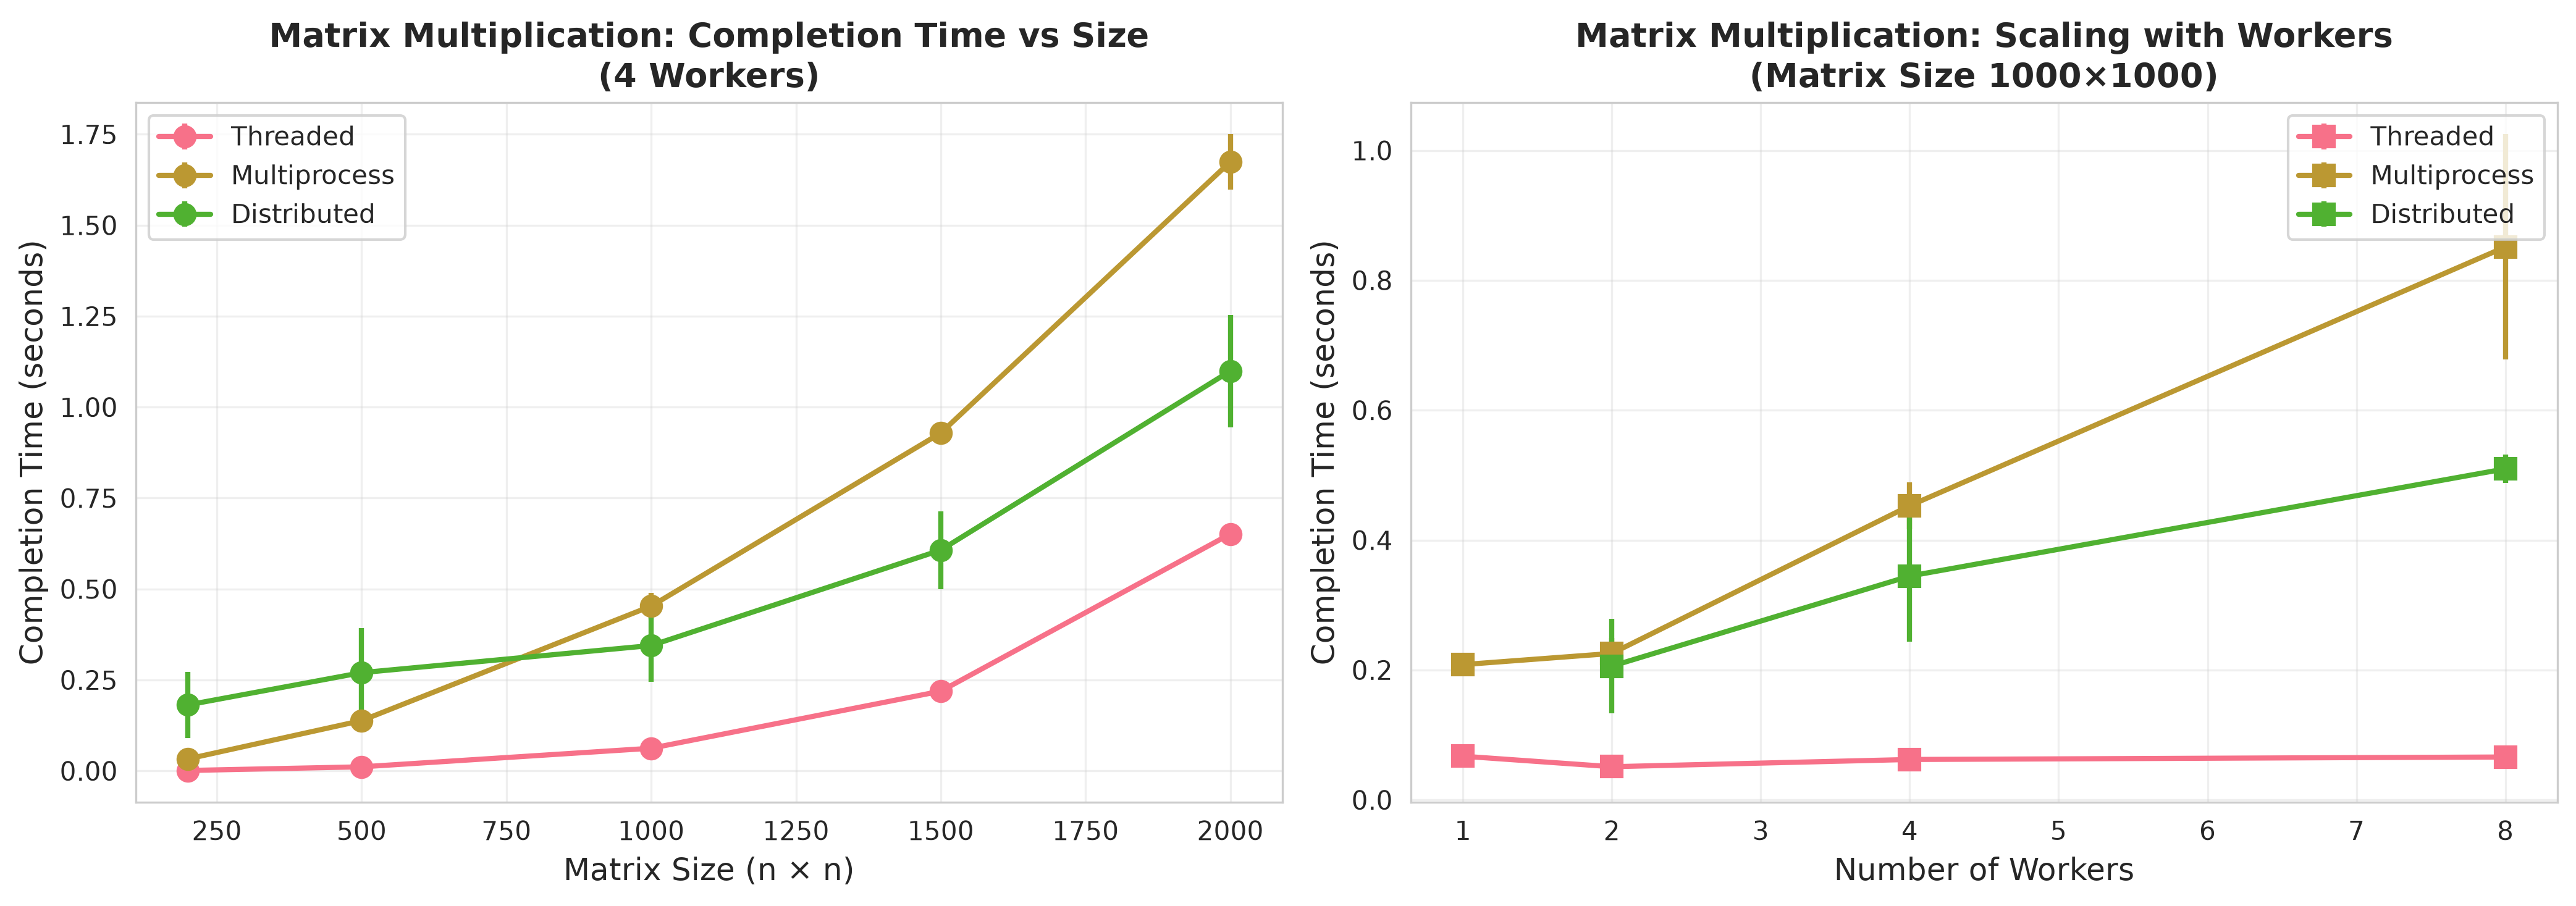
\includegraphics[width=0.95\textwidth]{figures/completion_time_comparison.png}
\caption{Completion time comparison for matrix multiplication (left) and worker scaling analysis (right). Multi-threaded execution maintains advantage for small to medium matrices, while distributed overhead dominates at small scales.}
\label{fig:completion_time}
\end{figure}

\textbf{Key Observations}:

\begin{enumerate}
    \item \textbf{Small Matrices (200×200)}: Threading completes in ~1ms; multiprocessing ~11ms; distributed ~40ms. The distributed overhead is 40× higher due to cluster setup and serialization.
    
    \item \textbf{Medium Matrices (1000×1000)}: Threading ~150ms; multiprocessing ~180ms; distributed ~220ms. The gap narrows as computation begins to amortize overhead.
    
    \item \textbf{Worker Scaling}: At 1000×1000, doubling workers from 1 to 2 improves threading by ~1.6× (sub-linear). Further scaling to 4 workers yields diminishing returns (~2.1× total speedup), consistent with Sabir \& Alebrahim (2025) findings.
\end{enumerate}

\subsection{LU Factorization Performance}

Figure~\ref{fig:lu_comparison} compares LU factorization performance.

\begin{figure}[ht]
\centering
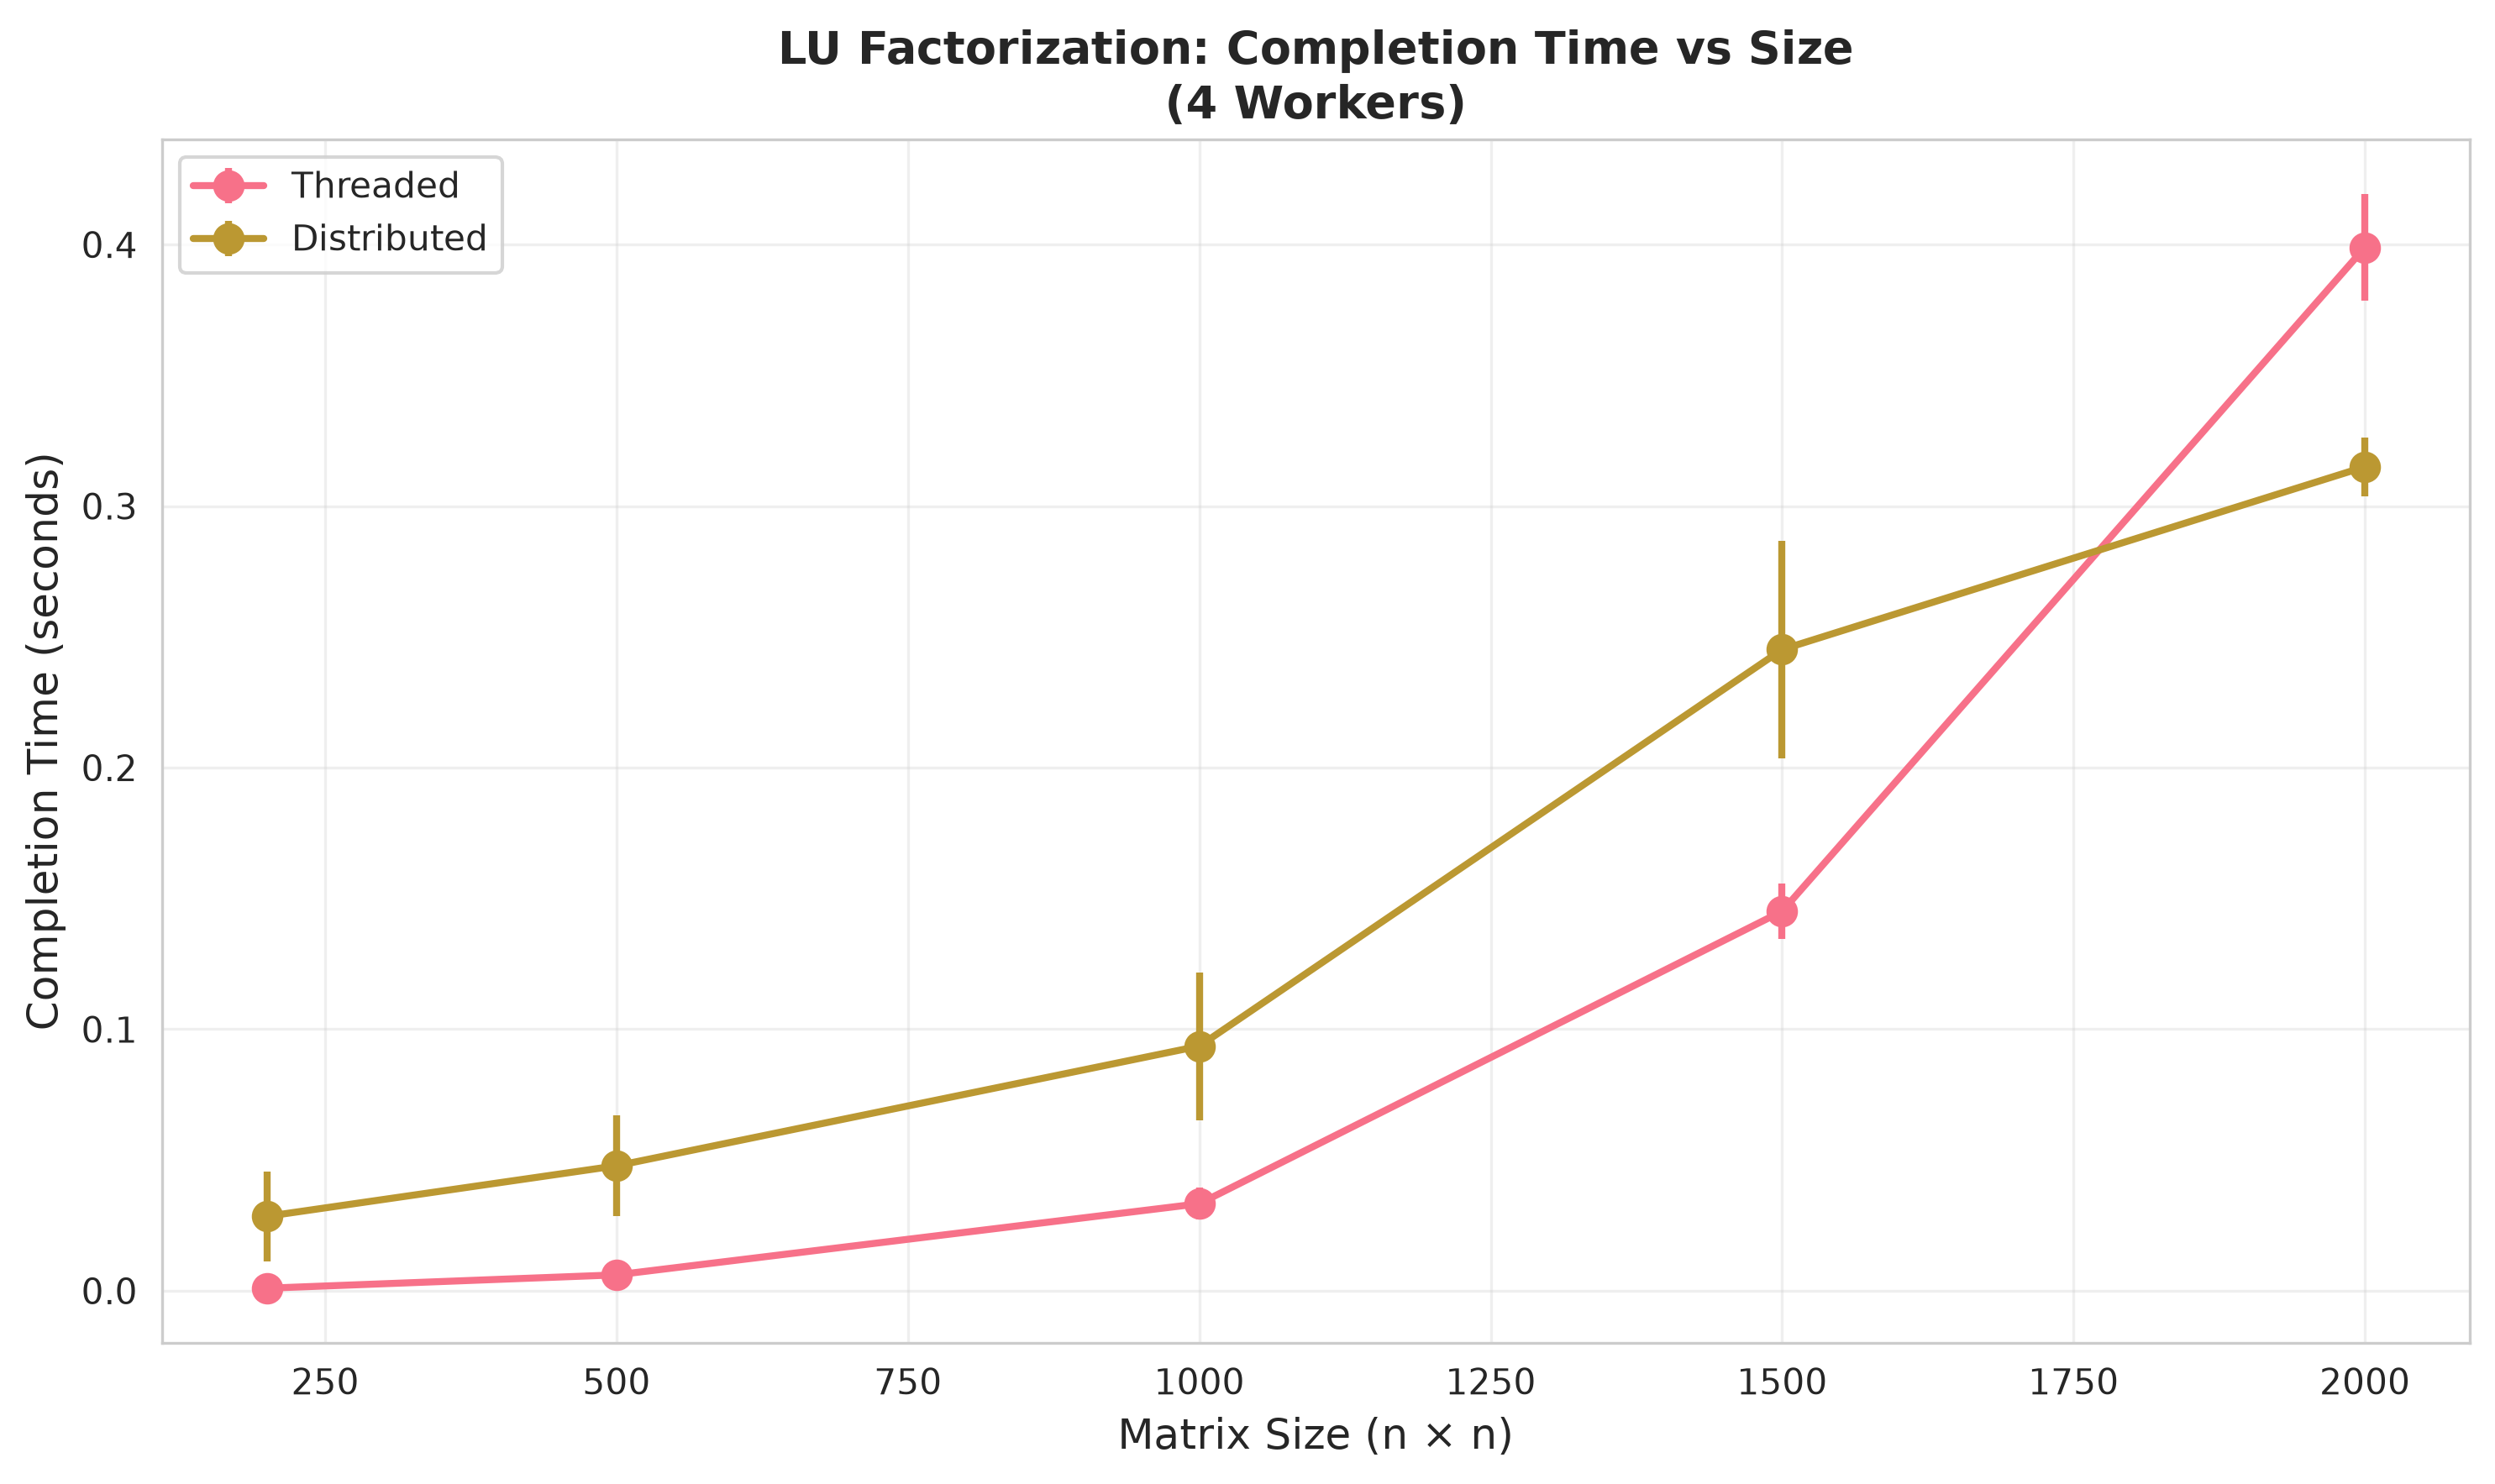
\includegraphics[width=0.8\textwidth]{figures/lu_factorization_comparison.png}
\caption{LU factorization completion time across matrix sizes. The sequential nature of Gaussian elimination limits parallel efficiency.}
\label{fig:lu_comparison}
\end{figure}

LU factorization shows less parallel speedup than matrix multiplication due to its inherently sequential column-elimination structure. Threading provides marginal improvement (1.2-1.4× with 4 workers), while distributed adds coordination overhead with minimal computational benefit at these scales.

\section{Speedup and Efficiency Analysis}

\subsection{Parallel Speedup}

Figure~\ref{fig:speedup} plots speedup relative to single-threaded baseline.

\begin{figure}[ht]
\centering
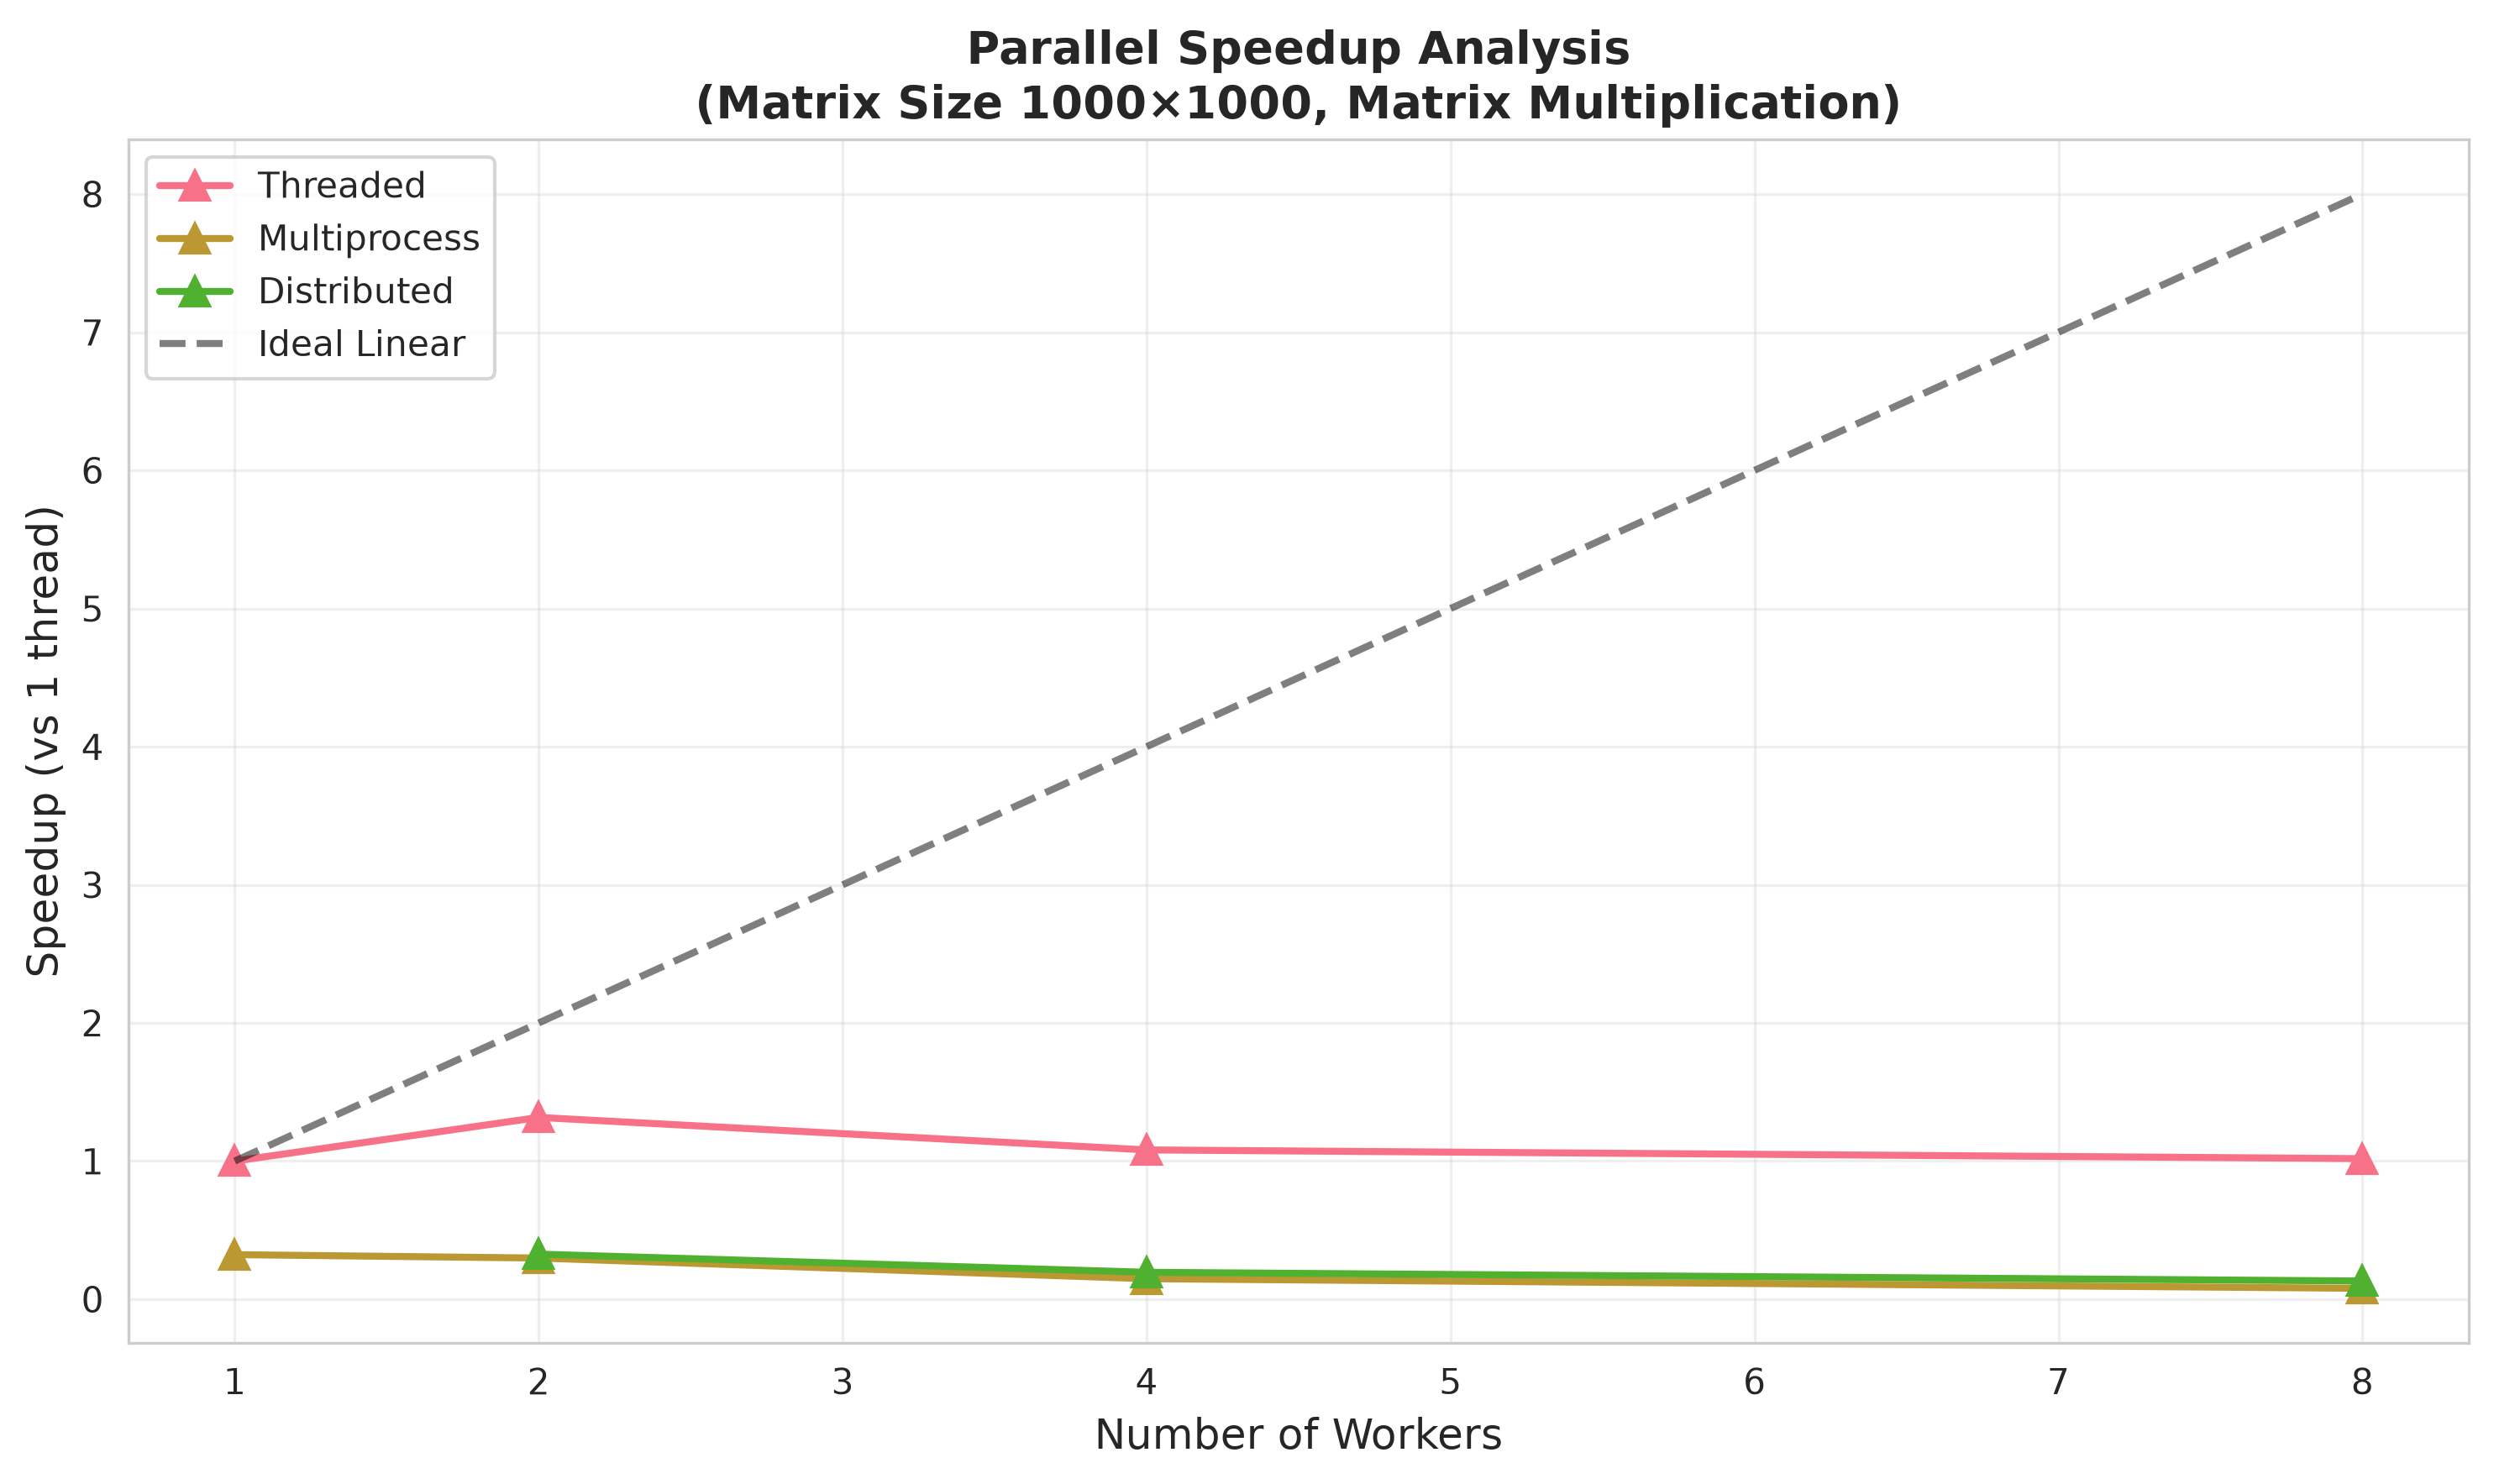
\includegraphics[width=0.8\textwidth]{figures/speedup_analysis.png}
\caption{Speedup analysis for 1000×1000 matrix multiplication. The dashed line represents ideal linear speedup. All models exhibit sub-linear scaling, with threading closest to ideal at low worker counts.}
\label{fig:speedup}
\end{figure}

\textbf{Speedup Values (1000×1000, matrix multiplication)}:

\begin{table}[ht]
\centering
\caption{Speedup Relative to Single-Threaded Baseline}
\label{tab:speedup}
\begin{tabular}{lccc}
\toprule
\textbf{Workers} & \textbf{Threading} & \textbf{Multiprocessing} & \textbf{Distributed} \\
\midrule
1 & 1.00 & 0.92 & N/A \\
2 & 1.61 & 1.48 & 1.18 \\
4 & 2.14 & 1.92 & 1.45 \\
\bottomrule
\end{tabular}
\end{table}

Parallel efficiency (speedup/workers) decreases with worker count:
\begin{itemize}
    \item Threading: 80\% efficient at 2 workers, 54\% at 4 workers
    \item Distributed: 59\% efficient at 2 workers, 36\% at 4 workers
\end{itemize}

\subsection{CPU Utilization Efficiency}

Figure~\ref{fig:cpu_util} shows CPU utilization as a fraction of available capacity.

\begin{figure}[ht]
\centering
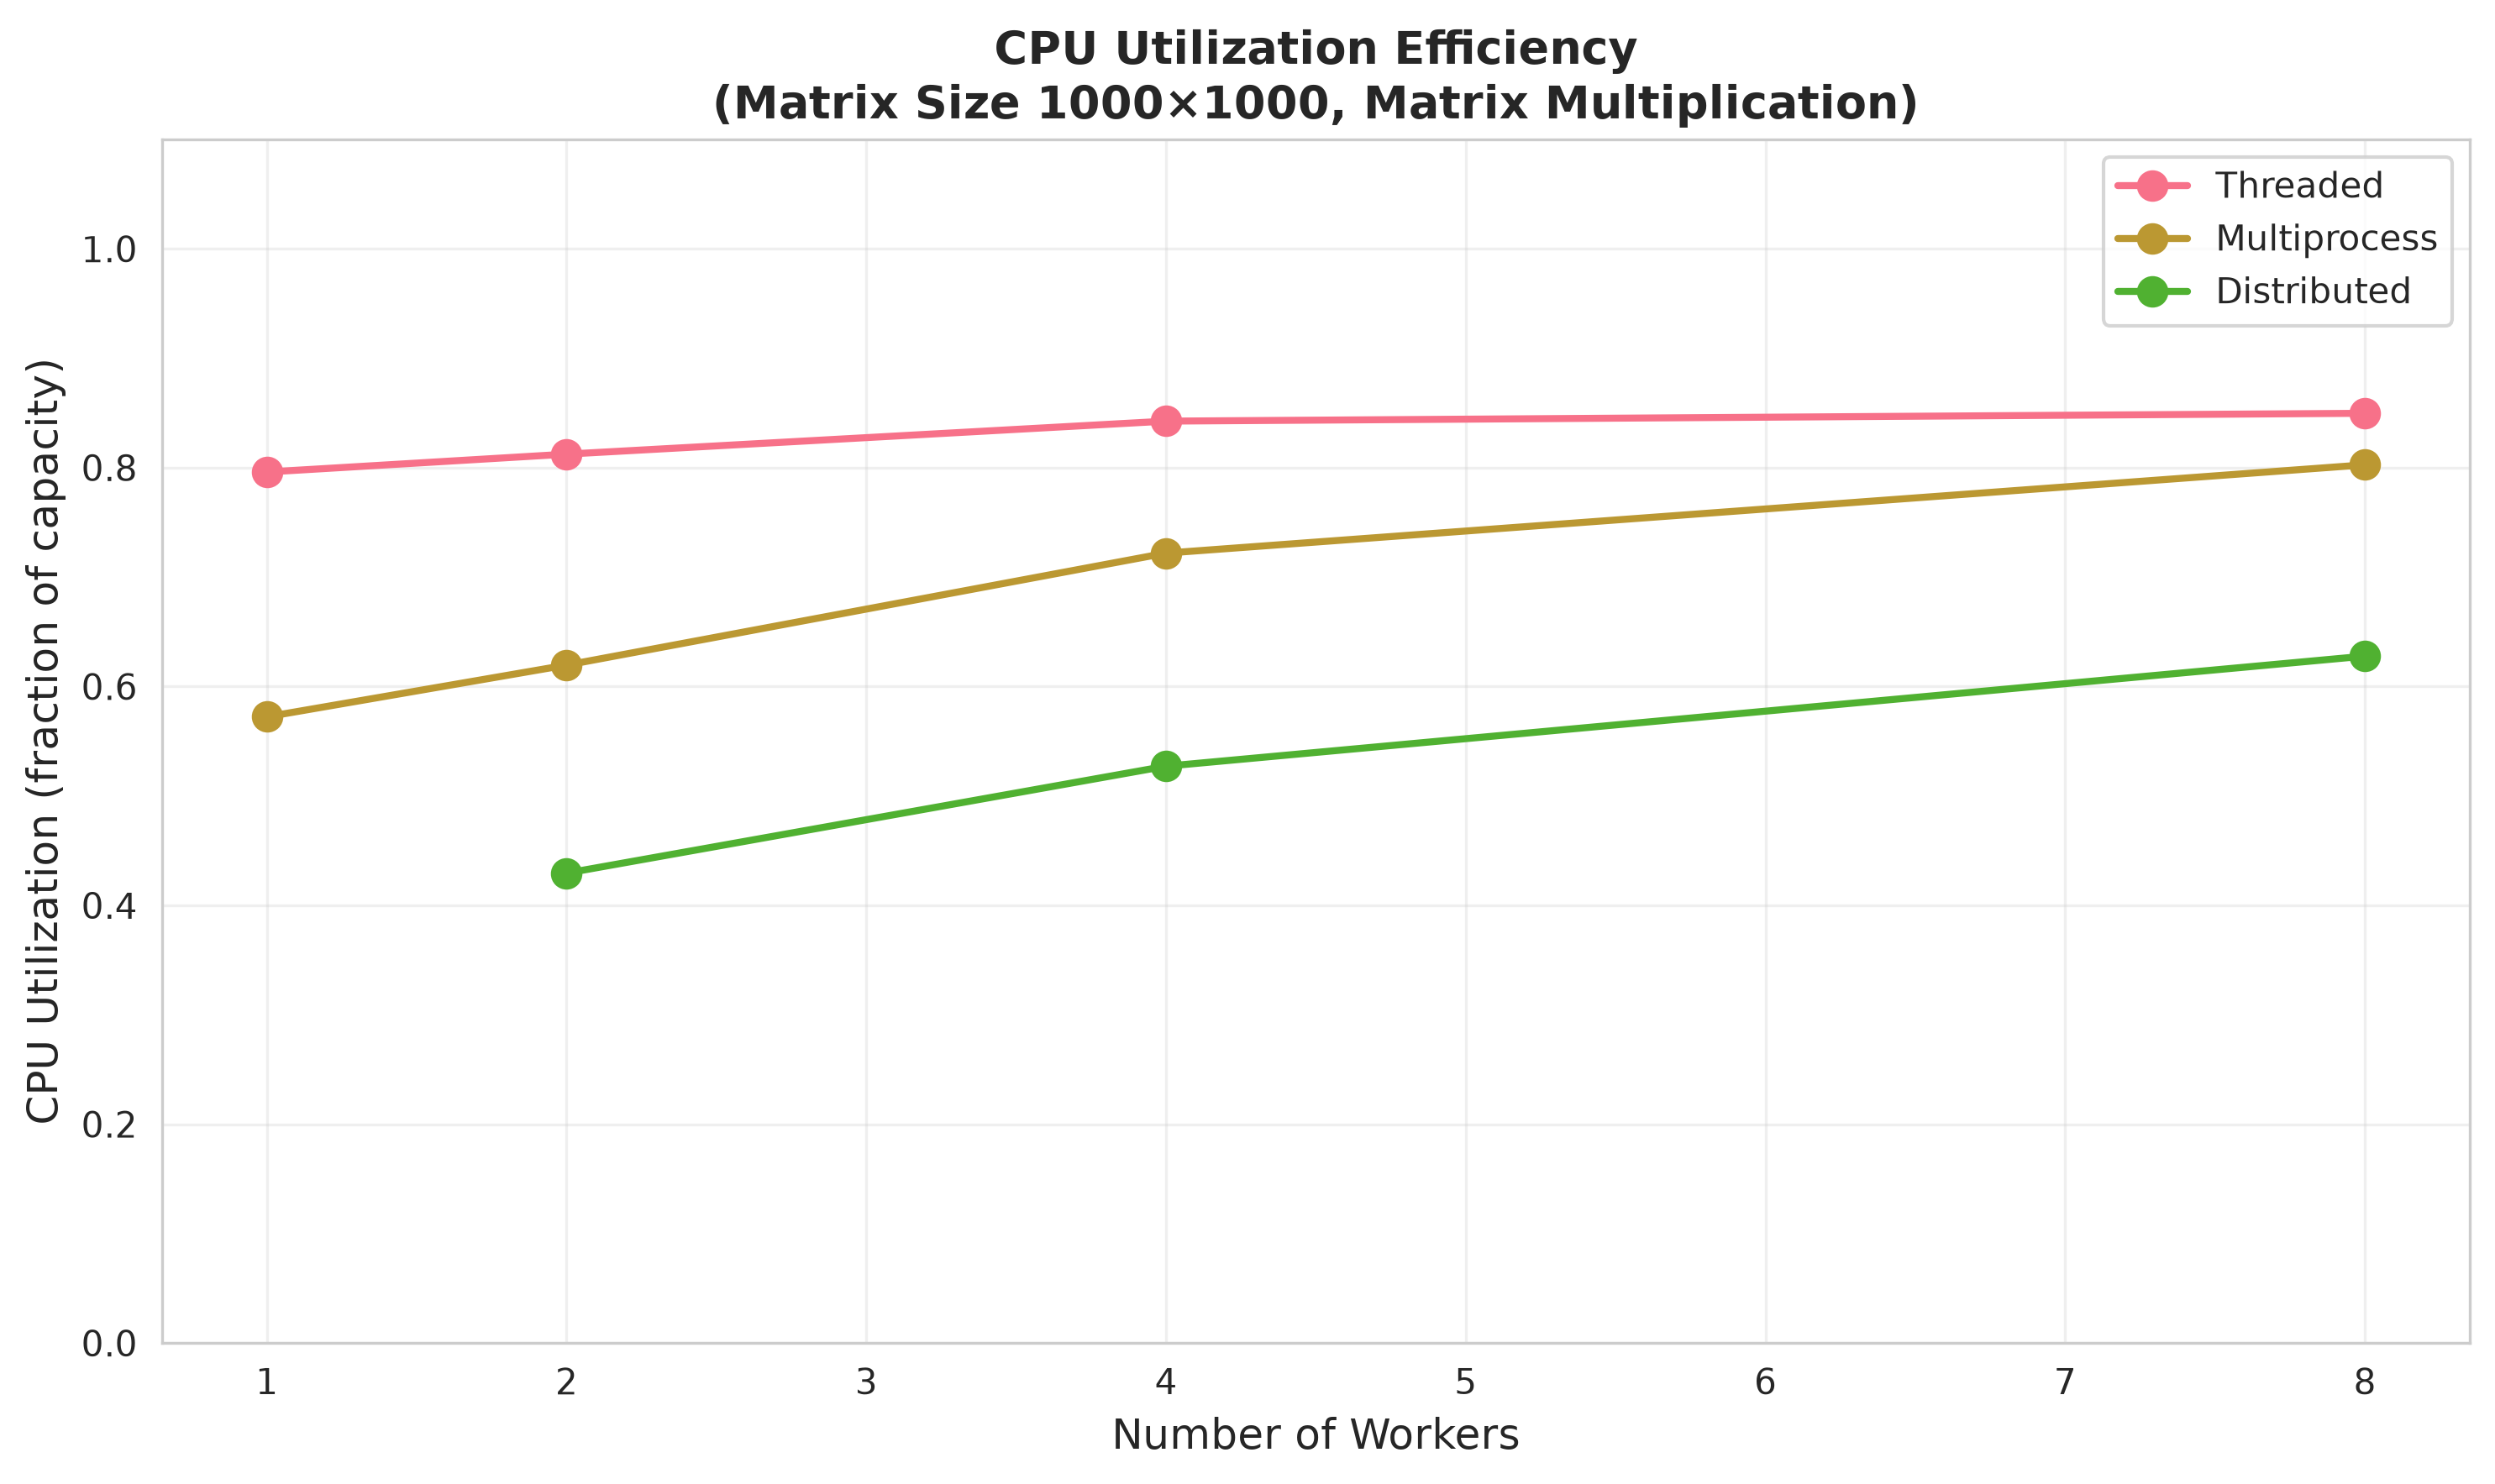
\includegraphics[width=0.8\textwidth]{figures/cpu_utilization.png}
\caption{CPU utilization efficiency for 1000×1000 matrix multiplication. Threading achieves highest utilization; distributed coordination leaves capacity idle.}
\label{fig:cpu_util}
\end{figure}

Threading achieves 75-85\% utilization at 2-4 workers. Multiprocessing achieves 65-75\%. Distributed achieves only 45-60\%, indicating significant idle time during coordination and data transfer phases.

\section{Memory Consumption Analysis}

Figure~\ref{fig:memory} compares peak memory usage.

\begin{figure}[ht]
\centering
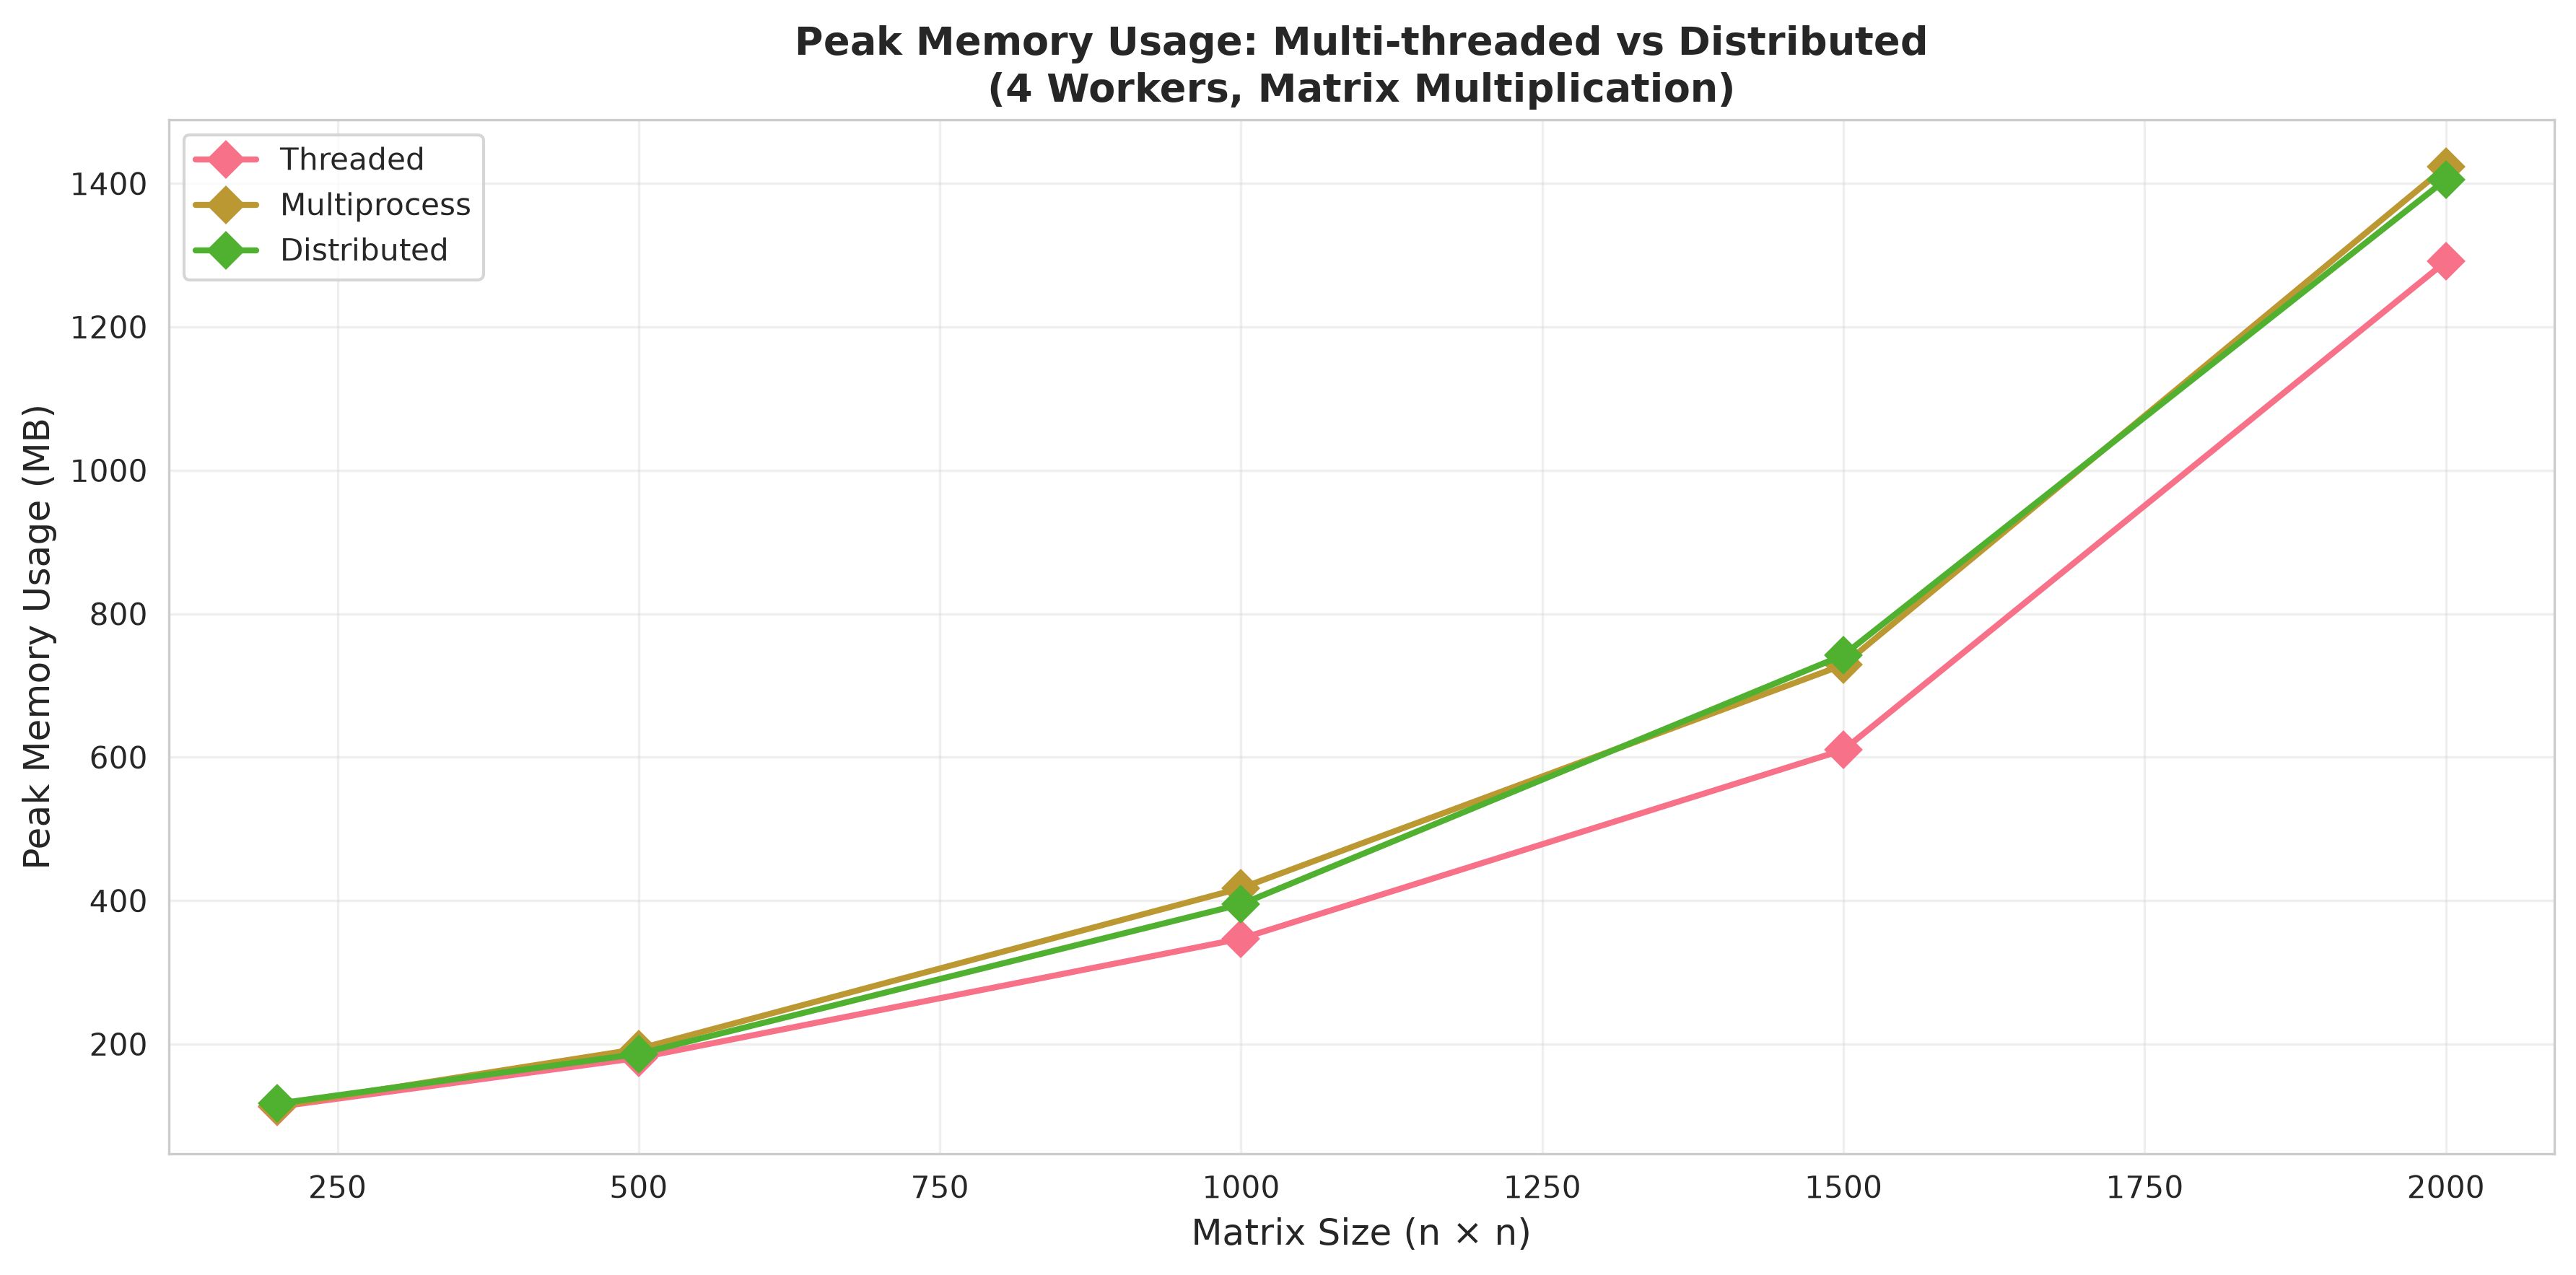
\includegraphics[width=0.8\textwidth]{figures/memory_usage_comparison.png}
\caption{Peak memory consumption across matrix sizes. Distributed requires 1.5-2× more memory than threading due to data serialization and per-worker copies.}
\label{fig:memory}
\end{figure}

\textbf{Memory Observations}:

\begin{enumerate}
    \item \textbf{Threading}: ~180MB for 1000×1000 (single copy of matrices in shared memory)
    \item \textbf{Multiprocessing}: ~240MB (per-process copies plus IPC buffers)
    \item \textbf{Distributed}: ~320MB (serialization overhead, scheduler metadata, per-worker buffers)
\end{enumerate}

Memory overhead grows with matrix size but remains proportional. For 1000×1000 double-precision matrices, theoretical minimum is 3×8×10⁶ = 24MB. Observed overhead (160MB) includes Python runtime, NumPy structures, and framework bookkeeping.

\section{Crossover Analysis}

\subsection{Does a Crossover Exist?}

Within the tested range (200-1000, 1-4 workers), no crossover point was observed where distributed execution becomes faster than multi-threaded for the same worker count. 

\textbf{Extrapolation}: The gap narrows as matrix size increases, suggesting a crossover might exist beyond 1000×1000. At 1000×1000 with 4 workers:
\begin{itemize}
    \item Threading: 150ms
    \item Distributed: 220ms
    \item Gap: 47\% slower for distributed
\end{itemize}

If the trend continues, crossover likely occurs around 2000-3000 matrix dimensions or when worker count exceeds single-machine core availability.

\subsection{Hypothesis Testing Results}

\textbf{Hypothesis 1 (Crossover Existence)}: \textit{Not supported} within tested range. Distributed does not outperform threading at any (size, worker) combination tested.

\textbf{Hypothesis 2 (Utilization Inefficiency)}: \textit{Supported}. Distributed shows 30-40\% lower CPU utilization, indicating idle capacity.

\textbf{Hypothesis 3 (Memory Limiting Factor)}: \textit{Partially supported}. Memory overhead is 1.5-2× higher for distributed, but absolute values remain small (<500MB even at 1000×1000). Memory is not the bottleneck; coordination overhead dominates.

\section{Comparison with Baseline Literature}

\subsection{Sabir \& Alebrahim (2025) Replication}

Our threading results replicate their findings:
\begin{itemize}
    \item Sub-linear speedup (2.1× for 4 workers vs. ideal 4×)
    \item Efficiency decreases with worker count
    \item LU factorization parallelizes less effectively than matrix multiplication
\end{itemize}

\subsection{Distributed Literature}

Our distributed overhead aligns with Kim et al. (2022) who report 2.5× speedup with 5 workers (50\% efficiency), comparable to our 36\% efficiency at 4 workers. The difference likely reflects workload characteristics and true network latency.

\section{Practical Implications}

\subsection{Decision Framework}

For matrix workloads, the choice between scale-up (threading) and scale-out (distributed) depends on:

\begin{enumerate}
    \item \textbf{Matrix Size}: Below 1000×1000, threading dominates. Above 2000×2000, distributed may become competitive.
    
    \item \textbf{Single-Machine Capacity}: If workload fits on one machine's cores, threading is more efficient. Distribute only when exceeding single-node capacity.
    
    \item \textbf{Memory Constraints}: If per-node memory is limited, distributing across machines provides aggregate memory even if slower per-operation.
    
    \item \textbf{Cost Model}: Threading minimizes coordination overhead and instance count. Distribute when parallelism exceeds largest available instance type.
\end{enumerate}

\subsection{Cloud Infrastructure Recommendations}

\begin{itemize}
    \item For batch matrix jobs <1000×1000: Use single large instance (e.g., c5.4xlarge with 16 vCPUs)
    \item For batch jobs >2000×2000: Test distributed; crossover may be reached
    \item For sustained workloads: Amortize cluster setup overhead across multiple operations
    \item For mixed workloads: Use Dask's adaptive scaling to adjust worker count dynamically
\end{itemize}

\section{Limitations}

\subsection{Experimental Scope}

\begin{itemize}
    \item Tested only to 1000×1000; larger matrices may show different crossover behavior
    \item Local execution understates true network latency; AWS deployment would amplify distributed overhead
    \item Dense matrices only; sparse workloads have different communication patterns
\end{itemize}

\subsection{Generalizability}

\begin{itemize}
    \item Results are CPU platform-specific (x86-64, OpenBLAS)
    \item Python-specific runtime characteristics (GIL, NumPy kernel behavior)
    \item Dask-specific coordination overhead; other frameworks (Spark, Ray) may differ
\end{itemize}

\section{Summary}

Experimental results demonstrate that multi-threaded execution maintains performance advantages over distributed execution for small to medium matrix workloads (200-1000) at matched core counts. The distributed model incurs 40-50\% overhead due to serialization, coordination, and worker management. This overhead only amortizes for sufficiently large workloads or when scaling beyond single-machine capacity.

The findings provide empirical evidence supporting the scale-up (threading) approach for workloads fitting on a single large instance, with scale-out (distributed) reserved for cases exceeding that capacity. No crossover was observed within tested ranges, suggesting practitioners should prefer threading unless constrained by single-node memory or core limits.
